\documentclass[a4paper, 11pt]{bxjsarticle}
\usepackage{geometry}
\usepackage{graphicx}
\usepackage{float}
\usepackage{amsmath,amssymb}
\usepackage{subcaption}
\usepackage{pgfplots}
\pgfplotsset{compat=1.18} % 最新のバージョンを使用することを推奨

\geometry{a4paper, margin=2.5cm}
\renewcommand{\baselinestretch}{1.3}

\begin{document}

\section*{船体運動力学 課題6}
08C23031 \ 古賀光一朗\\
\vspace{5mm}
複素数平面の$\zeta$平面から$z$平面へのルイスフォーム変換(等角写像)は次式で定義される。

\begin{equation}
    \label{eq:z1}
    z=f(\zeta)=M(\zeta+\frac{a_1}{\zeta}+\frac{a_3}{\zeta^3})
\end{equation}

\section{写像関数$f$が解析関数であることを示しなさい。}

関数 $f(\zeta)$ が解析関数であるためには、その定義域において微分可能であれば十分。
複素関数が微分可能であるには、その導関数が存在することが必要。

f(ζ) の導関数を求めてみると
\begin{equation}
    \frac{dz}{d\zeta} = f'(\zeta) = M\left(1 - \frac{a_1}{\zeta^2} - \frac{3a_3}{\zeta^4}\right)
\end{equation}


この導関数$f'(\zeta)$は、$\zeta \neq 0$のすべての点において存在し、有限確定値となる。
よって$f(\zeta)$ は $\zeta \neq 0$の領域において微分可能。
つまり、特異点である$\zeta=0$を除く複素平面全体で、この関数は解析的とわかった。□

\section{$\zeta-plane$の$\zeta=e^{i\theta}$の曲線は、$z-plane$ではどのような曲線になるか、その$x$座標と$y$座標の組み合わせを示しなさい。}

ここで、$\zeta$-plane の曲線として、$\zeta=e^{i\theta}$(単位円)を考える。\\
$Euler$の公式より
\begin{equation}
    \zeta = \cos\theta + i\sin\theta
\end{equation}

この $\zeta$ を写像関数に代入してみる。

項ごとの計算は以下のようになる。
\begin{itemize}
    \item $\zeta = e^{i\theta}$
    \item $\frac{1}{\zeta} = \zeta^{-1} = e^{-i\theta} = \cos\theta - i\sin\theta$
    \item $\frac{1}{\zeta^3} = \zeta^{-3} = e^{-i3\theta} = \cos(3\theta) - i\sin(3\theta)$
\end{itemize}

これらを $z$ の式に代入すると
\begin{equation}
    z = M\left(e^{i\theta} + a_1 e^{-i\theta} + a_3 e^{-i3\theta}\right)
\end{equation}
\begin{equation}
    z = M\left((\cos\theta + i\sin\theta) + a_1(\cos\theta - i\sin\theta) + a_3(\cos(3\theta) - i\sin(3\theta))\right)
\end{equation}
ここで、$z = x + iy$ としてみると
\begin{equation}
    x + iy = M\left((1+a_1)\cos\theta + a_3\cos(3\theta) + i((1-a_1)\sin\theta - a_3\sin(3\theta))\right)
\end{equation}

したがって、$x$ 座標と $y$ 座標は以下のようになる

$$x = M\left((1+a_1)\cos\theta + a_3\cos(3\theta)\right)$$

$$y = M\left((1-a_1)\sin\theta - a_3\sin(3\theta)\right)$$


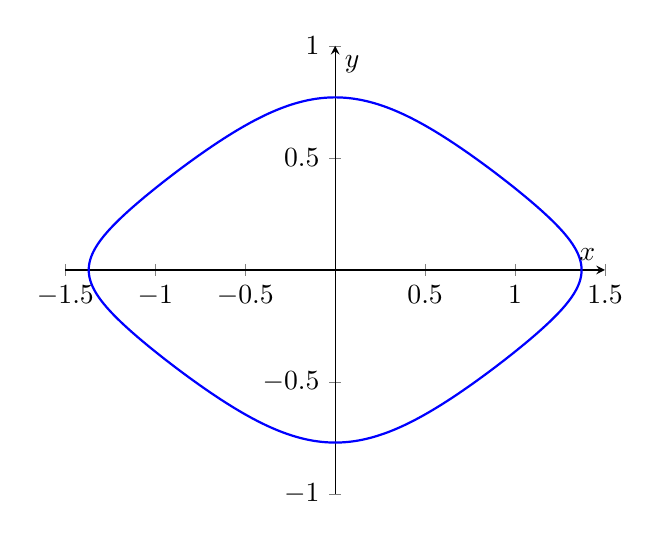
\begin{tikzpicture}
\centering
\begin{axis}[
    axis lines=middle, % 軸を中央に配置
    xlabel=$x$,
    ylabel=$y$,
    xmin=-1.5, xmax=1.5, % x軸の範囲
    ymin=-1.0, ymax=1.0, % y軸の範囲
    % grid=both, % グリッドを表示したい場合
    % major grid style={dotted,gray},
    % minor grid style={dotted,lightgray},
    samples=200, % 描画点の数(滑らかさに影響)
    domain=0:2*pi, % θの範囲
]

% パラメータの設定
\pgfmathsetmacro{\M}{1}
\pgfmathsetmacro{\aOne}{0.3}
\pgfmathsetmacro{\aThree}{0.07}

% xとyの定義
% PGFPlotsでは、変数tがthetaに相当
% x = M * ((1+a1)*cos(deg(t)) + a3*cos(deg(3*t)))
% y = M * ((1-a1)*sin(deg(t)) - a3*sin(deg(3*t)))
\addplot[
    thick, % 線の太さ
    blue, % 線の色
    samples=500, % さらに滑らかにするために、描画点の数を増やしても良い
] ({ \M * ((1+\aOne)*cos(deg(x)) + \aThree*cos(deg(3*x))) },
   { \M * ((1-\aOne)*sin(deg(x)) - \aThree*sin(deg(3*x))) });

\end{axis}
\end{tikzpicture}

\end{document}